{\scalefont{0.45}
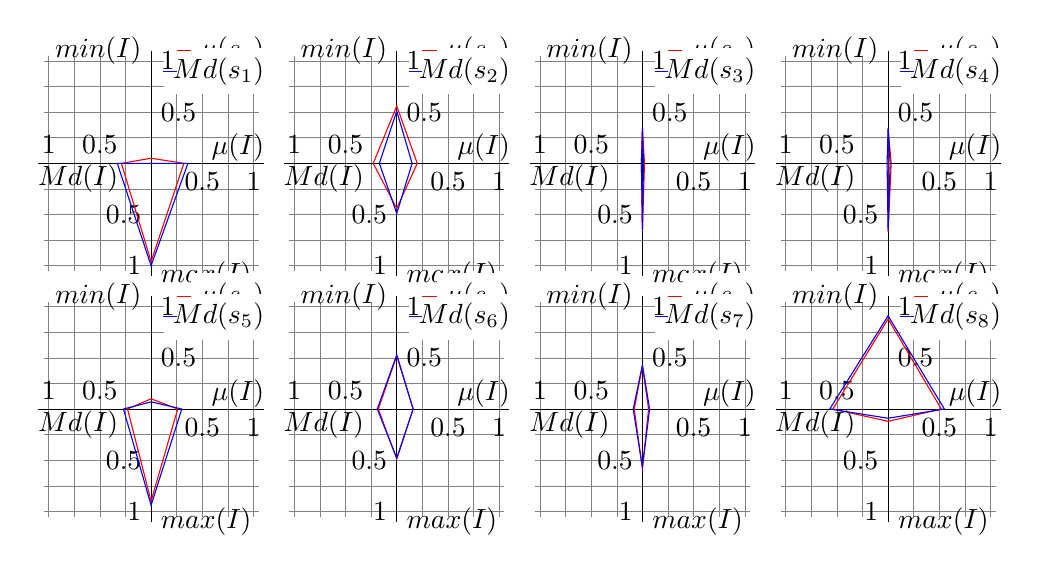
\begin{tikzpicture}[node distance=3mm, scale=1.3]
\def\lengthAxis{1.1}
\def\AxisSpace{2.4}


\def\MeanElements{{{0.32,0.05,0.29,0.96}}, {{0.20,0.56,0.23,0.44}}, {{0.02,0.35,0.01,0.66}}, {{0.03,0.34,0.00,0.67}}, {{0.26,0.10,0.23,0.90}}, {{0.16,0.52,0.18,0.49}}, {{0.06,0.42,0.08,0.58}}, {{0.52,0.88,0.54,0.12}}}

\def\MedianElements{{{0.36,0.00,0.33,1.00}}, {{0.15,0.51,0.17,0.49}}, {{0.01,0.35,0.01,0.65}}, {{0.02,0.35,0.01,0.66}}, {{0.30,0.07,0.27,0.94}}, {{0.16,0.53,0.19,0.48}}, {{0.07,0.43,0.09,0.57}}, {{0.55,0.91,0.57,0.09}}}

\foreach \elementPoints [count=\i] in \MeanElements {
\pgfmathsetmacro{\x}{\AxisSpace*mod(\i-1,4)}
\pgfmathsetmacro{\y}{-1*\AxisSpace*int((\i-1)/4)}

\draw[step=0.25,gray,very thin, shift={(\x,\y)}] (-1.05,-1.05) grid (1.05,1.05);

\path (\x,\y)	+ (  		 \lengthAxis,              		      0)	coordinate (meanI)
                        + (  -1*\lengthAxis,          		       	  0)	coordinate (medI) 
					    + (                    	  0, 		\lengthAxis	)	coordinate (minI) 
					    + (                     	  0,  -1*\lengthAxis)	coordinate (maxI)
					    + (					 0.25,						  0)	coordinate (legendRef);

\draw 	(meanI) 	+(.1,.15) 	node[anchor=east] 	{$\mu(I)$}
		    (medI) 	+(-.1,-.15)	node[anchor=west]	{$Md(I)$}
		    (minI)		node[left] 				{$min(I)$}
		    (maxI)		node[right]			{$max(I)$};

 \draw ({\x+.1},\y) 	+(\lengthAxis,\lengthAxis)			node[fill=white,anchor=east] (mulabel){$\mu(s_\i)$}
					   				+(\lengthAxis,{\lengthAxis-.2})	node[fill=white,anchor=east] (medlabel){$Md(s_\i)$};

\draw[color=red] (mulabel.west) -- (mulabel.west -| legendRef);
\draw[color=blue] (medlabel.west) -- (medlabel.west -| legendRef);
		      
\draw[thin] (meanI) -- (medI) (minI) -- (maxI);

%\draw[thin] (\x,\y)	+ (	   1,	   0)	circle [radius=1pt] node[below]	{1}
%                        		+ (	  -1, 	   0)	circle [radius=1pt] node[above]	{1}
%							    + (      0,     1)	circle [radius=1pt] node[right] 		{1}
%							    + (  	   0,	  -1)	circle [radius=1pt] node[left]		{1}
%							    + (	0.5,	   0)	circle [radius=1pt] node[below]	{0.5}
%                        		+ ( -0.5,	   0)	circle [radius=1pt] node[above]	{0.5}
%							    + (	   0,	0.5)	circle [radius=1pt] node[right] 		{0.5}
%							    + (	   0, -0.5)	circle [radius=1pt] node[left]		{0.5};

\draw[thin] (\x,\y)	+ (	   1,	   0)	node[below]	{1}
                        		+ (	  -1, 	   0)	node[above]	{1}
							    + (      0,     1)	node[right] 	{1}
							    + (  	   0,	  -1)	node[left]		{1}
							    + (	0.5,	   0)	node[below]	{0.5}
                        		+ ( -0.5,	   0)	node[above]	{0.5}
							    + (	   0,	0.5)	node[right] 	{0.5}
							    + (	   0, -0.5)	node[left]		{0.5};

  \draw[color=red] (\x,\y) +(   \elementPoints[0],                    0)
                -- +(                   0,    \elementPoints[1])
                -- +(-1*\elementPoints[2],                    0)
                -- +(                   0, -1*\elementPoints[3])
                -- cycle;
  }
  
\foreach \elementPoints [count=\i] in \MedianElements {
\pgfmathsetmacro{\x}{\AxisSpace*mod(\i-1,4)}
\pgfmathsetmacro{\y}{-1*\AxisSpace*int((\i-1)/4)}
\draw[color=blue] (\x,\y) +(   \elementPoints[0],                    0)
                -- +(                   0,    \elementPoints[1])
                -- +(-1*\elementPoints[2],                    0)
                -- +(                   0, -1*\elementPoints[3])
                -- cycle;
  }
\end{tikzpicture}

}